% platex, uplatex 両対応.
\ifdefined\ucs
  %\documentclass[uplatex, report, a4j]{jsbook}
  \documentclass[uplatex, 12pt, papersize]{jsbook}
\else
  %\documentclass[report, a4j]{jsbook}
  \documentclass[12pt, papersize]{jsbook}
\fi


% =================================================== %
\def\emph#1{\textbf{\em{#1}}} 
%-----------------------------------------------------------------%
\makeatletter% @付きのコマンドが使えるようにする。
%ファイル末尾で \makeatother で最後で解除すること
%-----------------------------------------------------------------%

% パッケージ読み込み部:開始
% 有用そうなのをいくつか列挙しておきます.
% 他にも様々あります.
%   参考URL:http://www.biwako.shiga-u.ac.jp/sensei/kumazawa/texindex.html

% 画像挿入用パッケージ: graphicx
% 文字等に色づけする場合に必要: color
% 
%   画像の利用方法 (png, jpg/jpeg, pdf、などが利用できる)
%   例 
%     \begin{figure}
%       \includegraphics[width=10cm,bb=0 0 600 600]{image/sample.png}
%     \end{figure}
%
%   注
%     []にて指定している値は,[表示横幅, bb=0 0 画像横pixel数 画像縦pixel数]です.
%     bb=以後は,ebbコマンドなどでsample.bbを作成しておけば不要です.
%     Windows : makebb.bat
%     @echo on
%      for %%i in (*.png)  do ebb %%i
%      for %%i in (*.pdf)  do ebb %%i
%      for %%i in (*.jpg)  do ebb %%i
%      for %%i in (*.jpeg) do ebb %%i
%
%     Linux / MacOSX : makebb.sh
%      #!/bin/sh -e
%      cd `dirname "$0"`
%      xbb *.pdf *.png *.jpg *.jpeg && ls *xbb | \
%      perl -ne 'chomp; ~s/\.xbb//g; print "mv $_.xbb $_.bb\n"' | \
%      sh 
%
% =======
%
\usepackage[dvipdfmx]{graphicx, color}

% 背景にすかし文字 (DRAFT) を表示 : pdfdraftcopy : graphicx に依存
%   提出用と間違えるのを予防
%   開発元URL: http://sarovar.org/projects/pdfdraftcopy/
%
% IsDraft が \def されている場合だけ有効
\@ifundefined{IsDraft}{}{\usepackage[watermark]{pdfdraftcopy}
\watermarkgraphic{images/draft_copy.pdf}}

% ブロックコメント
% \begin{comment} \end{comment}
\usepackage{comment}

% しおりの作成、目次や参考文献をクリッカブルリンクへ
% いろいろなパッケージと互換性問題があるようなので,他のパッケージを利用する場合にはチェックすること
% 依存関係情報: http://oku.edu.mie-u.ac.jp/~okumura/texwiki/?hyperref#z442922c
%
\usepackage[dvipdfm
	, bookmarks=true
	, bookmarksopen=true
 	, bookmarksnumbered=true
	, CJKbookmarks=true
%
	, backref=true
	, pdfborder={0 0 0} % width
%
	, colorlinks=false
	, frenchlinks=false
%	, linkbordercolor={1 1 1} % RGB
%	, citebordercolor={1 1 1} %RGB
%	, urlbordercolor={1 1 1} %RGB
%	, pdfhighlight=/I
]{hyperref}
% しおりの文字化け解消.必要な文字コード指定を入れる.
%\AtBeginDvi{\special{pdf:tounicode 90ms-RKSJ-UCS2}}% SJIS 
%\AtBeginDvi{\special{pdf:tounicode EUC-UCS2}} % EUC
%\AtBeginDvi{\special{pdf:tounicode UTF8-UCS2}} % UTF-8
%
% 文字コードを自動判定してしおりの文字化けを解消できるパッケージ.
% 上のオプションをオフにしてこちらを使ってもよい.
\usepackage{pxjahyper}
%
% PDFのメタ情報を設定したければ以下を追加
%\hypersetup{
%	pdftitle={タイトル},
%	pdfsubject={小見出し},
%	pdfauthor={PDF制作者名},
%	pdfkeywords={キーワード1; キーワード2; キーワード3;},
%}

% urlをそのまま表記可能にする.
%   本来であれば><%#^~などはエスケープしないといけない
%   また、1 word として認識されるために、自動で折り返してくれないURLを、
%   途中で折り返しをしてくれる。
%
% 使い方:
%    \url{http://www.ubi.cs.ritsumei.ac.jp}
%    \url{<a href=``http://www.ubi.cs.ritsumei.ac.jp''>Link</a>}
\usepackage{url}
\urlstyle{rm}
% 数式パッケージ
%   美文書作成などを参照してください.
%\usepackage{amsmath, amssymb}

% 表用パッケージ
%   きれいな表が書けます.
%   参考URL: http://www.biwako.shiga-u.ac.jp/sensei/kumazawa/tex/hhline.html
\usepackage{hhline, multirow}

% 表の見栄えを良くする
% 表の架線が上下だけ太くなります.
%   参考URL: http://www.biwako.shiga-u.ac.jp/sensei/kumazawa/tex/booktabs.html
\usepackage{booktabs}

% いろいろな囲み線作成用
%   様々な場面で利用できます.便利です.
%   参考URL: http://www.biwako.shiga-u.ac.jp/sensei/kumazawa/tex/fancybox.html 
%   参考URL: http://www.biwako.shiga-u.ac.jp/sensei/kumazawa/tex/ascmac.html
\usepackage{fancybox, ascmac}

% 可換図を書けるように
%   参考URL: http://www.biwako.shiga-u.ac.jp/sensei/kumazawa/tex/amscd.html
% \usepackage{amscd}

%% 以下、私作のコマンド
\usepackage{here}
\usepackage{bm}

%
% \TS{hoehoge}: パラグラフのトピックセンテンスを指定
% \listofts: トピックセンテンスを抽出してリスト化: 目次のような感じ
%
% \TODO{}: TODO を出力 (赤色で TODO: hogehoge)
% \listoftodo: TODOを抽出してリスト化: 目次のような感じ
%
%%%%%%%%%%%%%%%%%%%%%%%%%%%%%%%%%%%%%%%%%%%%%
%
\def\RED#1{{\color{red}#1}}%
%
\def\TS#1{\AddToContLine{lots}{#1}#1}%
\newcommand{\listtsname}{Paragraph Topic Sentenses (\RED{for Debug})}%
\newcommand{\listofts}{\listof{ts}}%
%
\newcommand{\TODO}{\secdef\@TODO\@sTODO}%
\def\@TODO[#1]#2{\@sTODO{#2}\@ifundefined{PrintTodo}{}{\\}}%
\def\@sTODO#1{\AddToContLine{lotodo}{#1}\@ifundefined{PrintTodo}{}{\RED{TODO: #1}}}% started TODO means [ \TODO*{hogehoge} ]
\newcommand{\listtodoname}{List of TODO (\RED{for Debug})}%
\newcommand{\listoftodo}{\@ifundefined{PrintTodo}{}{\listof{todo}}}%
\newcommand{\forceListoftodo}{\listof{todo}}%
%
%
%%%%%%%%%%%%%%%%%%%%%%%%%
\def\listof#1{%
  \if@twocolumn\@restonecoltrue\onecolumn%
  \else\@restonecolfalse\fi%
  \abstract{{\csname list#1name\endcsname}}%
  \@mkboth{{\csname list#1name\endcsname}}{}%
  \@starttoc{lo#1}%
  \if@restonecol\twocolumn\fi%
}%
\def\AddToContLine#1#2{%
\@ifundefined{c@atcl#1}{\newcounter{atcl#1}[chapter]}{}%
\ifnum \csname c@atcl#1\endcsname =0 % chapter用のダミーを追加
  \refstepcounter{atcl#1}%
  \addcontentsline{#1}{chapter}{\protect\numberline{\@chapapp\thechapter\@chappos}}%
\fi%
\ifnum \c@section>0 %
  \ifnum \c@subsection >0 %
    \ifnum \c@paragraph >0 %
      \ifnum \c@subparagraph >0 %
        \AddToContLineSec{#1}{subparagraph}{#2}%
      \else\AddToContLineSec{#1}{paragraph}{#2}\fi%
    \else\AddToContLineSec{#1}{subsection}{#2}\fi%
  \else\AddToContLineSec{#1}{section}{#2}\fi%
\else%
  \ifnum \csname c@atcl#1\endcsname >0 %
    \addcontentsline{#1}{section}{\protect\numberline{}#2}%
  \else%
    \refstepcounter{atcl#1}%
    \addcontentsline{#1}{chapter}{\protect\numberline{\@chapapp\thechapter\@chappos}#2}%
  \fi%
\fi%
}%
\def\AddToContLineSec#1#2#3{%
  \@ifundefined{c@atcl#2#1}{\newcounter{atcl#2#1}[#2]}{}
  \ifnum \csname c@atcl#2#1\endcsname >0 %  各セクションの一番始めで無ければ章番号無し
    \addcontentsline{#1}{#2}{\protect\numberline{}#3}%
  \else%
    \refstepcounter{atcl#2#1}%  セクションの一番始めであれば章番号付き
    \addcontentsline{#1}{#2}{\protect\numberline{\csname the#2\endcsname}#3}%
  \fi%
}%
%
\def\BoldFirstRef#1#2{\@ifundefined{c@#1}{\newcounter{#1}\textbf{#2}}{#2}}%
\@ifundefined{figref}{\def\figref#1{\BoldFirstRef{figref#1}{図 \ref{#1}}}}{}% 図出力
\@ifundefined{tabref}{\def\tabref#1{\BoldFirstRef{tabref#1}{表 \ref{#1}}}}{}% 表出力
\@ifundefined{secref}{\def\secref#1{\ref{#1} 節}}{}%
\@ifundefined{chapref}{\def\chapref#1{第 \ref{#1} 章}}{}%
\def\SetJsDescriptionIndent#1{%
%%%%%%%%%%%%%%%%%%%%%%%%%%%%%
\renewenvironment{description}{%
  \list{}{%
    \leftmargin=#1
    \labelwidth=\leftmargin
    \labelsep=1zw
    \advance \labelwidth by -\labelsep
    \let \makelabel=\descriptionlabel}}{\endlist}
%%%%%%%%%%%%%%%%%%%%%%%%%%%%%
}%
\def\abstract#1{%
\chapter*{#1}\@mkboth{#1}{}%
\@ifundefined{c@abstract}{\newcounter{abstract}\pagenumbering{roman}}{}%
}%
\def\startMain{%
\if@openright\cleardoublepage\else\clearpage\fi%
\pagenumbering{arabic}%
}
%-----------------------------------------------------------------%
%-----------------------------------------------------------------%
%
%
\def\BachelorThesis{卒 業 論 文}
\def\MasterThesis{修 士 論 文}
\def\DoctoralThesis{博 士 論 文}
\def\@thesisTitle{圧力センサ搭載ヘルメットを用いた\\本人認証手法の提案}
\def\@thesisSupervisor{卒業研究3 (1O):双見 京介,村尾 和哉 担当} % 卒業研究3のクラス名と担当教員名を記載
%\def\@thesisSupervisor{卒業研究3 (1H):西尾 信彦 担当}
\def\@thesisKind{\MasterThesis}
\def\@thesisYear{2019年}
%\def\@thesisYear{2019年}
%\def\@thesisEraName{平成XX年}
\def\@thesisSemester{秋学期} % 秋か春を記載
%\def\@thesisSemester{秋学期}
\def\@thesisAuther{藤井 敦寛}
\def\@thesisNameOfGraduateSchool{立命館大学大学院}
\def\@thesisNameOfUnderGraduate{立命館大学 情報理工学部}
\def\@thesisNameOfMajor{情報理工学研究科情報理工学専攻}
\def\@thesisNameOfGrade{情報システム学科 4回生 2600160357-3} % 2017年度入学者はコース名に変更
%\def\@thesisNameOfGrade{情報システム学科 4回生 2600xxxxxxxx}
\def\thesisTitle#1{\gdef\@thesisTitle{#1}}
\def\thesisKind#1{\gdef\@thesisKind{#1}}
\def\thesisYear#1{\gdef\@thesisYear{#1}}
\def\thesisEraName#1{\gdef\@thesisEraName{#1}}
\def\thesisAuther#1{\gdef\@thesisAuther{#1}}
\def\thesisNameOfGraduateSchool#1{\gdef\@thesisNameOfGraduateSchool{#1}}
\def\thesisNameOfMajor#1{\gdef\@thesisNameOfMajor{#1}}
\def\makeThesisTitle{
\begin{titlepage}%
\centering
\begin{minipage}[]{\fullwidth}
\large
 

% 表紙の配置や文字のサイズは以下で調整
\vspace{6mm}
{\@thesisYear}度({\@thesisSemester})\\
{\@thesisSupervisor}\\%
\begin{center}
\vspace{2mm}
{\Large {\@thesisKind}}\\
\vspace{27mm}
%
{\LARGE {\@thesisTitle}}\\%
\vspace{84mm}%
{\@thesisNameOfUnderGraduate}\\%
%{\@thesisNameOfGraduateSchool}\\%
{\@thesisNameOfGrade}\\%
%{\@thesisNameOfMajor}\\%
%
\vspace{7mm}%
{\Large {\@thesisAuther}}%
\end{center}%
\end{minipage}%
\end{titlepage}%
}
%
%-----------------------------------------------------------------%
\makeatother%
%-----------------------------------------------------------------%
 % 普段使っているパッケージいろいろ
% =================================================== %
%
% subsection まで目次に出力
\setcounter{tocdepth}{2}

\begin{document}
\pagenumbering{roman}

\thesisKind{\BachelorThesis} % \BachelorThesis or \MasterThesis or \DoctoralThesis

\makeThesisTitle

\abstract{要旨}
近年,四輪車において広く普及しているスマートキーシステムが,徐々に二輪車でも採用されつつある.しかし,このシステムは電子キーを所持しておく必要があり,キーを紛失する恐れや,キーの盗難による車両盗難のリスクがある.そこで,ヘルメットをキーの代用とすることが可能であれば,二輪車のヘルメットロックに装備しておくことで,所有者は身体一つで乗車が可能となる.また,先述のリスクも回避できると考えた.個人識別の手法として,デバイスを二輪車の車両に取り付ける手法は,走行時の衝撃からの耐久性などの問題が生じる.そのため,ヘルメットにデバイスを装着して識別が可能である手法を選択する必要がある.さらに,デバイスが軽量かつ視界を遮らないという条件を満たさなければならない.これらの条件を考慮し,本研究では圧力センサを搭載したヘルメットを装着することで個人識別を行う手法を提案する.識別には特徴があり複製が難しいものとして頭部形状を使用した.また,頭部状態の測定にヘルメットを用いている先行研究は筆者らの知る限りは存在しない.そのため,提案手法は頭部装着型デバイスとして新規性がある.提案手法は,ヘルメットに搭載した32個の圧力センサから得られたセンサ値をベクトルとして扱い,事前に登録フェーズで蓄積しておいた所有者のセンサデータ群とのマハラノビス距離を計算し,閾値を用いて識別を行う.本手法で用いるデバイス,およびソフトウェアを設計,実装し評価実験を行った.プロトタイプデバイスは市販のフルフェイス型のヘルメットを加工し圧力センサを取り付け,マイコンに配線することで実装した.解析用のソフトウェアはPythonのscikit-learnのsklearn.covariance.MinCovDetを使用してマハラノビス距離を計算し,閾値を移動しながら評価指標であるFRR,FAR,EERを求めるよう設計した.ソフトウェアを実装した後,評価用に被験者9人からそれぞれ2秒間のセンサ値を20回分収集した.これらのデータセットからマハラノビス距離を用いて識別を行う.5分割交差検証を行い,被験者全員の平均EERが約7.8\%という結果が得られた.

\tableofcontents % 目次
\listoffigures % 図目次
\listoftables % 表目次

%本文開始
\startMain

\chapter{はじめに}
\label{introduction}
近年,販売されている四輪車の多くにスマートキーシステムを導入している.スマートキーシステムとは,電子キーをポケットなどに入れて接近すると電波を感知しドアの施錠や解錠,エンジンの始動をボタン一つで操作できるようにする機能である.このシステムは二輪車においても導入されつつある.二輪車におけるスマートキーシステムも同様に,電子キーを所持しておくことで,キーシリンダーにキーを挿し込む手間なくラゲッジスペースと呼ばれる荷物を収納するスペースの解錠やエンジンの始動が可能になる機能である.しかしながら,このシステムではキーを所持しておかなければならず,キーを紛失する恐れやキーの盗難による車両盗難のリスクがある.\par
本研究では,圧力センサを搭載したヘルメットを装着することで,頭部形状に基づき個人識別をする手法を提案する.二輪車での走行で必要であるヘルメットを用いた本人認証が実現できれば,既存のキーに関する問題点を解決できると考えられる.予め車両とリンクしておいたヘルメットをキーの代わりとして二輪車のヘルメットロックに装備しておく.そうすれば,利用者は身体一つで乗車できるため,キーの紛失のリスクを減少させることができる.利用者はヘルメットを被ることで個人認証をして,車両の持ち主がヘルメットを被った場合はエンジンの始動を可能にする.一方で,車両の持ち主以外がヘルメットを被った場合はエンジンの始動ができないようにすることで,車両盗難のリスクも減少させることができる.\par
個人認証の要素には各個人ごとに特徴があり,かつ複製が難しい身体部位を用いる必要がある.当麻ら\cite{face}が提案しているステレオカメラを用いた顔認証システムでは,少数のカメラで顔認証が行える方法が提案されている.顔認証は二輪車にあらかじめ取り付けておいたカメラを用いて,ヘルメット装着前にカメラの方を向くことで実装可能だと考えられる.しかし,カメラに対して屋外の過酷な環境への耐久性が求められる.近年,普及されつつある個人認証方法として指紋認証があげられる.指紋認証をヘルメットに搭載することも可能であるが,越前ら\cite{finger_print}の研究のように,指紋は写真などから簡単に複製されてしまうリスクを持つ.本研究で用いる頭部形状は人により異なる特徴が存在する.また,身体部位としても大きいため,複製するには大掛かりな器具が必要になることが想定される.以上の理由から,個人認証の要素に有効であると考えられるため頭部形状を用いる手法を提案する.\par
以降,\ref{related}章では関連研究を紹介する.\ref{method}章では提案手法,\ref{make}章では実装について述べる.\ref{evaluation}章では提案手法の評価実験の結果を述べつつ考察を行う.最後に\ref{conclude}章で本研究をまとめる.
\chapter{Related Work}
\label{sec:related}
In this chapter, I introduce research on sensing with wearable devices, the use of smartwatches, and the use of pulse data.

% 2.1
\section{Sensing with Wearable Devices}
There is much research on wearable devices that are worn on body parts, and devices of various shapes have been investigated. Ham et al. \cite{smart_wristband} proposed a wristband-type device as an input device for smart glasses. The device is equipped with a touch panel and an inertial measurement unit, and it can be operated by touch or with a motion such as a twist of the wrist. Because the device is simply worn on the wrist, it offers a high degree of freedom by not restricting the user's movement. A touch panel is used for pointing to improve the input stability. Hernandez et al. \cite{bioglass} proposed a method for acquiring the pulse rate and respiration rate from data obtained from the accelerometer, gyroscope, and camera built into Google Glass, a head-mounted wearable device. Nishajith et al. \cite{smart_cap} designed and implemented ``Smart Cap,'' a wearable device to assist the visually impaired with situational awareness. The device consists of a Raspberry Pi 3, a Raspberry Pi NoIR Camera v2 (an infrared camera module for the Raspberry Pi), an earphone, and a power supply. The infrared camera obtains an image, and the object detected in the image is described by voice through the earphone.\par

For a non-optical approach, Bello et al. \cite{MoCapaci} proposed a wearable system that detects body postures and gestures without requiring sensors to be firmly fixed to the body or integrated into a tight-fitting garment. They implemented a prototype, ``MoCaBlazer,'' by using a standard men's blazer, and they conducted evaluation experiments with 14 subjects. For recognition of 20 actions, the system achieved average recognition accuracy of 97.18\% for leave-one-recording-out evaluation and 86.25\% for user-independent recognition.\par

Among research on other sensor modalities, Vargas et al. \cite{Brainwear} developed an open-source electroencephalography (EEG) sensing module with a state-of-the-art analog front end that is pin- and protocol-compatible with popular ecosystems in the wearable and DIY communities. The goal was to facilitate broad use of EEG sensing in multimodal smart garments. They conducted an evaluation experiment with a proof-of-concept application of the system in a normal baseball cap. They concluded that the system achieved similar levels of recognition to those in other neuroscience studies with dedicated instruments. R\"{o}ddiger et al. \cite{earables} conducted a study with seven different commercially available ``earables'' that are targeted at daytime usage: to investigate their comfort and wearability during sleep, they were all worn by 14 study participants. The results showed that devices occupying more space in the outer ear canal with rigid parts are less desirable. Vekemans et al. \cite{MOTUS} implemented ``MOTUS,'' a prototype watch-back tactile display that conveys emotions, to explore the potential for emotional expression by applying tactile texture patterns to the wrist. A preliminary guessability study with the prototype showed agreement between the texture patterns and the users' interpretation of emotions. Zhou et al. \cite{CoRSA} developed ``CoRSA,'' a lightweight system that supplements existing sports apparel having cardiorespiratory monitoring capabilities with system-in-package (SiP) and system-on-chip (SoC) sensors, which are popular in the wearable computing community. Other studies have examined wearable devices based on rings \cite{wearable_ring1, wearable_ring2, TypingRing, ElectroRing}, belts \cite{wearable_belt1, SmartBelt, WaistonBeltX, wearable_belt2}, and masks \cite{wearable_mask1, wearable_mask2, SilentMask, Masquare}.\par

Various body parts have been investigated as locations for wearable devices, and researchers have sought to estimate the locations from sensor data. Vahdatpour et al. \cite{localization_vahdatpour} collected acceleration data during daily activities from 25 subjects who wore accelerometers at 10 locations on the forearm, upper arm, head, thigh, shin, and waist. From the collected data, a support vector machine (SVM) was able to estimate the attachment site with an average accuracy of 89\%. Sztyler et al. \cite{localization_sztyler} collected acceleration data during various physical activities from 15 subjects who had accelerometers attached to seven locations: the head, chest, left upper arm, left wrist, waist, left pants pocket, and left ankle. From the collected data, the attachment site was estimated with an average accuracy of 89\% by using a random forest. Kunze et al. \cite{localization_kunze} collected data during walking movements from six subjects who had accelerometers attached to four locations: the wrist, the right side of the head above the eye, the left pants pocket, and the left breast pocket. From the collected data, the attachment site was estimated using the C4.5 classifier. In addition, Yoshida et al. \cite{localization_yoshida} proposed a method to estimate the body part where a wearable device is attached without requiring the wearer to perform a specific action; instead, they used electrocardiography (ECG) and pulse data, which are biometric information that can be acquired by the wearable device.


% 2.2
\section{Studies on Smartwatches}
Among wearable devices, smartwatches have long been commercially available, and there is much research on them. Spinsante et al. \cite{accuracy_in_low_intensity} studied the heart rate obtained from a smartwatch during low-intensity physical activity and measured its accuracy. Sen et al. \cite{eating_recognition} proposed a method to record a user's eating behavior, such as the use of hands, chopsticks, or a spoon, by using data obtained from a smartwatch's accelerometer and gyroscope. By capturing food images with the smartwatch's built-in camera and performing image identification, the meal contents were also recorded. In another study, by leveraging the fact that smartwatches are always worn at the same location and in the same direction, Johnston et al. \cite{smartwatch_walk_authentication} proposed a method for biometric authentication based on gait data obtained from a smartwatch's accelerometer and gyroscope.\par

Smartphones are typically carried in a pants pocket or handbag, but compared to those locations, more activity information tends to be available at the wrist, where smartwatches are worn. Weiss et al. \cite{smartwatch_activity_recognition} showed that a smartwatch can identify actions more effectively than a smartphone in hand-based physical behaviors such as eating. The smartwatch could identify the behavior of ``drinking'' with 93.3\% accuracy, while the smartphone could only achieve 77.3\% accuracy.\par

Among other potential applications, Iakovakis et al. \cite{oh_detection} conducted a study on using a smartwatch to predict blood pressure drops due to postural changes. Orthostatic hypotension (OH) has been shown to cause dizziness and fainting and is a risk factor for falls in the young as well as the elderly. Accordingly, they proposed a mathematical prediction model that can reduce the risk of falls due to OH by sensing heart rate variability. Mauldin et al. \cite{smartfall} proposed an Android application, ``SmartFall,'' that detects falls by using acceleration data obtained from a commercially available smartwatch. The smartwatch is paired with a smartphone that runs the software. SmartFall communicates with a cloud server to perform the calculations necessary to predict falls in real time, while maintaining data privacy. Ciabattoni et al. \cite{smartwatch_stress_detection} proposed a method for detecting mental stress during various cognitive tasks in real time. Stress is classified by using galvanic skin response (GSR), RR interval (i.e., the time between successive R-peaks in an ECG), and body temperature data acquired by a commercial smartwatch. Sun et al. \cite{SleepMonitor} developed ``SleepMonitor,'' a smartwatch-based system for monitoring the user's respiratory rate and body position. The system uses accelerometer data collected at the wrist to estimate the respiratory rate. The results of evaluation experiments showed that the system could monitor the respiratory rate and body position during sleep with high accuracy under various conditions.\par

On the other hand, for an artificial limb, wearable devices cannot collect biometric information. In that case, methods using sensors such as accelerometers and gyroscopes are applicable, but methods using biometric data are not. Accordingly, I seek to make these applications available to users with artificial limbs as well as living limbs by inputting suitable data to the biometric sensors of wearable devices.


% 2.3
\section{Studies on Pulse Data}
Havriushenko et al. \cite{respiratory_rate_estimation1} proposed a method for estimating a user's respiratory rate from pulse wave data by using neural networks. The respiratory rate is often measured with a thermal sensor placed in the nasal channels or an elastic chest belt, but these devices may interfere with sleep. In contrast, their method can be implemented in a wearable device. The results of their evaluation showed an average respiratory rate estimation error lower than 2.2 breaths per minute. Jarchi et al. \cite{respiratory_rate_estimation2} proposed a method that relies on a nonlinear time-frequency representation, called the wavelet synchrosqueezed transform (WSST), to estimate the instantaneous respiratory rate from body-mounted PPG sensors. Han et al. \cite{arrhythmia_detection} proposed a method for detecting premature atrial contraction and premature ventricular contraction by using PPG data acquired from a smartwatch. Wang et al. \cite{alcohol_detection} developed a system for identifying excess alcohol consumption by using an SVM with data from ECG and PPG monitoring. Longmore et al. \cite{ppg_location} sought to identify a single location in the human anatomy for measuring simultaneously the heart rate (HR), blood oxygen saturation (SpO2), and respiration rate at rest and while walking by a single PPG sensor. In addition, Okamoto et al. proposed a method to recognize the arm's muscle activity state and a method to estimate a surface electromyogram (sEMG) from PPG data \cite{semg_okamoto}. The results of an evaluation experiment with five participants showed that three types of muscle activity were recognized with over 75\% accuracy, and the sEMG was estimated with an error of approximately 20\%.\par

Among potential pulse data applications related to emotions, Goshvarpour et al. \cite{emotion_recognition1} proposed a method for classifying emotional responses by means of a simple dynamic signal processing technique and a fusion framework. They recorded the ECG and finger pulse activity of 35 subjects during a rest condition and when the subjects were listening to music that was intended to stimulate certain emotions. After constructing Poincar\'e plots, an SVM was used to classify them into four emotions: happiness, sadness, peacefulness, and fear. Kajiwara et al. \cite{emotion_recognition2} developed an application for logistics companies that adopt a manual order picking system, given that emotions and engagement affect work efficiency and human errors. Specifically, they proposed a method for predicting emotions and engagement during work with a high exercise intensity from behavior and pulse wave data acquired by wearable devices. Pulse wave, eye movement, and general movement data are input to deep neural networks to estimate a worker's emotion and engagement. The results of verification experiments showed that the emotion and engagement during order picking could be accurately predicted from the worker's behavior with an error rate of 0.12 or less. Lee et al. \cite{emotion_recognition3} conducted research on improving the speed of emotion recognition by using a PPG signal. A two-dimensional emotion model based on valence and arousal was adopted, and a one-dimensional convolutional neural network (1D CNN) was used to recognize emotions from a 1.1-s PPG signal. The 1D CNN was tested as a binary classifier (high or low valence and arousal) by using the dataset for emotion analysis using physiological signals (DEAP), and it achieved recognition accuracies of 75.3\% for valence and 76.2\% for arousal. Udovi\v{c}i\'{c} et al. \cite{emotion_recognition4} studied emotion recognition using only GSR and PPG signals because of their suitability for implementation in a simple wearable device that can collect signals from a person without compromising comfort and privacy. In addition to the above studies, there have been many others on the use of PPG data for emotion recognition \cite{emotion_recognition5, emotion_recognition6, emotion_recognition7}.\par

Pulse data is one of the most important pieces of biological information, as it can be applied to detect abnormalities in the body and recognize emotions. Most pulse sensors in commercially available wearable devices use PPG. As a result, when a wearable device is mounted on an artificial limb, where there is no blood flow, pulse data cannot be acquired. Hence, among various kinds of biometric data, I focus on pulse data and propose a method to allow a wearable device to measure pulse data similar to that of a living limb even on an artificial limb.

\chapter{提案手法}
\label{method}
本章では提案手法の詳細を述べる.本研究はヘルメットをキーの代わりとして用いることを目標とし,圧力センサを搭載したヘルメットを装着して装着者の頭部形状を取得することで,個人識別を行う手法を提案する.\par
システム構成を図\ref{system}に示す.学習データ群および新たにプロトタイプデバイスから得られるデータは,32個のセンサ値であり32次元のベクトルとして扱う.提案するシステムではあらかじめ学習フェーズとして,所有者の頭部データを複数回収集しておく.このデータ群に対し,プロトタイプデバイスから得られたセンサ値のベクトルからのマハラノビス距離を計算する.マハラノビス距離とは統計学で用いられる一種の距離である.これは多次元のデータに対しても使用できる.データは32次元の連続ベクトルであり,学習フェーズで得られた多変数ベクトルのデータ列を
\[
  x^m = x_1, x_2, \ldots, x_m
\]
とすると,i番目のデータは
\[
  x_i = \left(
        \begin{array}{c}
            x_{i,1} \\
            x_{i,2} \\
            \vdots \\
            x_{i,32}
        \end{array}
    \right)
\]
と表すことができる.この平均値ベクトル$\mu$と分散共分散行列$\Sigma$は以下のように求められる.
\begin{eqnarray*}
  \mu &=& \frac{1}{m}\sum_{i=1}^{m}x_i \\
  \Sigma &=& \frac{1}{m}\sum_{i=1}^{m}(x_i-\mu)(x_i-\mu)^T
\end{eqnarray*}
このとき,学習データ群$x^m$に対する未知のユーザの入力データ$y$のマハラノビス距離は
\[
  D_{Mahalanobis} = \sqrt{(y-\mu)^{T}\Sigma^{-1}(y-\mu)}
\]
と定義される.ここで閾値を$\theta$と置き,
\[
  \theta < \sqrt{(y-\mu)^{T}\Sigma^{-1}(y-\mu)}
\]
を満たす場合,入力データ$y$は所有者以外の他人から得られた頭部データであると判定し異常値だとして拒否する.一方で,入力データ$y$に対して,
\[
  \theta \geq \sqrt{(y-\mu)^{T}\Sigma^{-1}(y-\mu)}
\]
を満たす場合,入力データ$y$は所有者本人から得られた頭部データであると判定し正常値だとして認証する.

\begin{figure}[!t]
  \begin{center}
    \includegraphics[width=1\linewidth]{figure/system.eps}
  \end{center}
  \caption{システム構成}
  \label{system}
\end{figure}
\chapter{実装}
\label{make}
\section{ハードウェア}
提案手法に用いる圧力センサを搭載したヘルメットを実装した.このデバイスの構成を図\ref{device},プロトタイプデバイスの全体図を図\ref{met_over}に示す.センサ値を正しく取得するには,センサとヘルメット装着者の頭部が密着している必要がある.そのため,フルフェイス型のB\&B社製BB100フルフェイスヘルメットを用いた.実装したプロトタイプデバイスの内部を図\ref{met_in}に示す.今回用いたヘルメットはフリーサイズであり,また内装の脱着が困難であった.そのため,頭頂部の内装を取り外して,新たに厚みのあるウレタンスポンジを取り付けた.図\ref{sensor}のようにウレタンスポンジの中央部に切り込みを入れ,インターリンク エレクトロニクス社製のFSR402,FSR402 ShortTailを挿し込むことで圧力センサを実装した.この圧力センサは頭頂部に4個,頭頂部周囲に16個,後頭部に6個,左右チークパッド部に6個の合計32個を搭載した.配線はヘルメットの頭頂部にドリルで穴あけ加工をし,ヘルメット外部に取り付けた10KΩの抵抗を配線してあるプリント基板を経由して,Arduino MEGA2560 R3の5V電源,GND,アナログ入力ポートに接続した.センサ1つあたりの回路図を図\ref{circuit}に示す.図\ref{circuit}に示した回路を図\ref{print}のプリント基板を通して32個並列に接続した.このプリント基板は取り外しが可能かつしっかりと固定するため,ヘルメットのシールド固定用に開けられたネジ穴を流用し,左頬部分にボルトで固定している.

\begin{figure}[!t]
  \begin{center}
    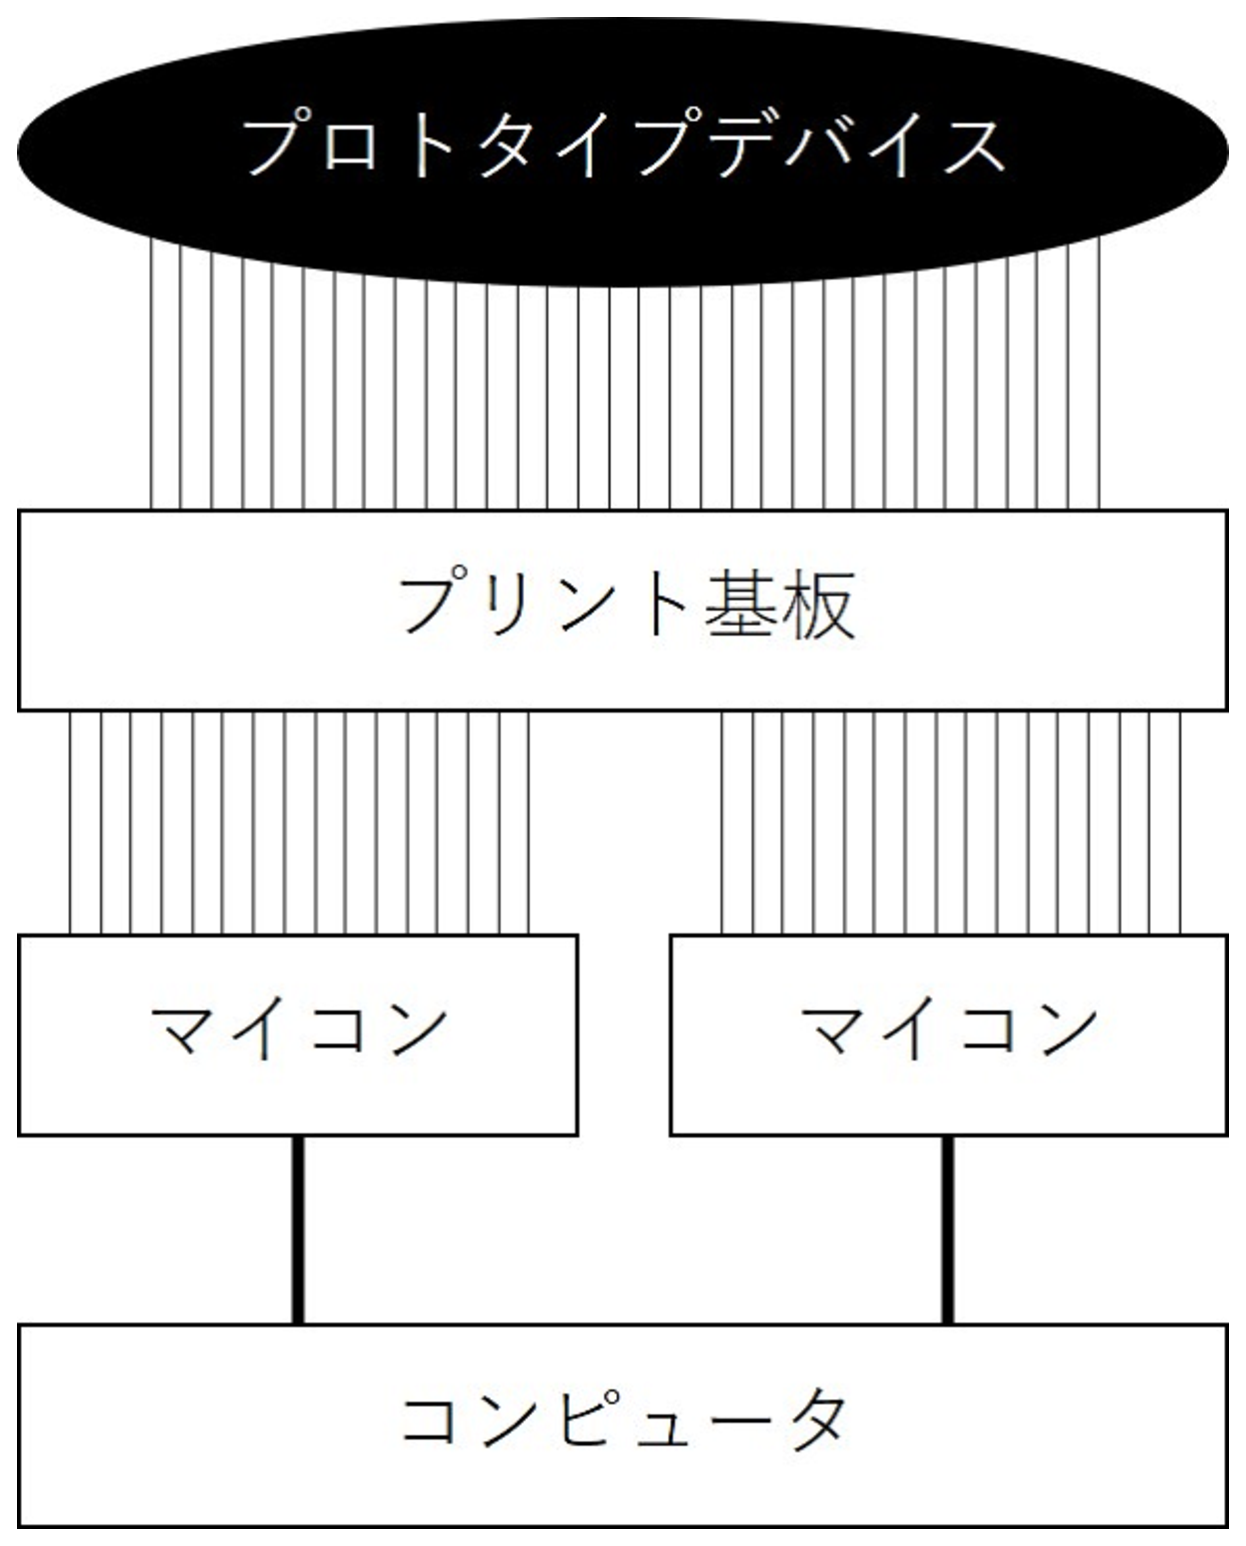
\includegraphics[width=0.5\linewidth]{figure/device.eps}
  \end{center}
  \caption{デバイス構成}
  \label{device}
\end{figure}

\begin{figure}[!t]
  \begin{center}
    \includegraphics[width=0.5\linewidth]{figure/met_over.eps}
  \end{center}
  \caption{プロトタイプデバイスの全体図}
  \label{met_over}
\end{figure}

\begin{figure}[!t]
  \begin{center}
    \includegraphics[width=0.5\linewidth]{figure/met_in.eps}
  \end{center}
  \caption{プロトタイプデバイスの内部}
  \label{met_in}
\end{figure}

\begin{figure}[!t]
  \begin{center}
    \includegraphics[width=0.5\linewidth]{figure/sensor.eps}
  \end{center}
  \caption{センサの実装方法}
  \label{sensor}
\end{figure}

\begin{figure}[!t]
  \begin{center}
    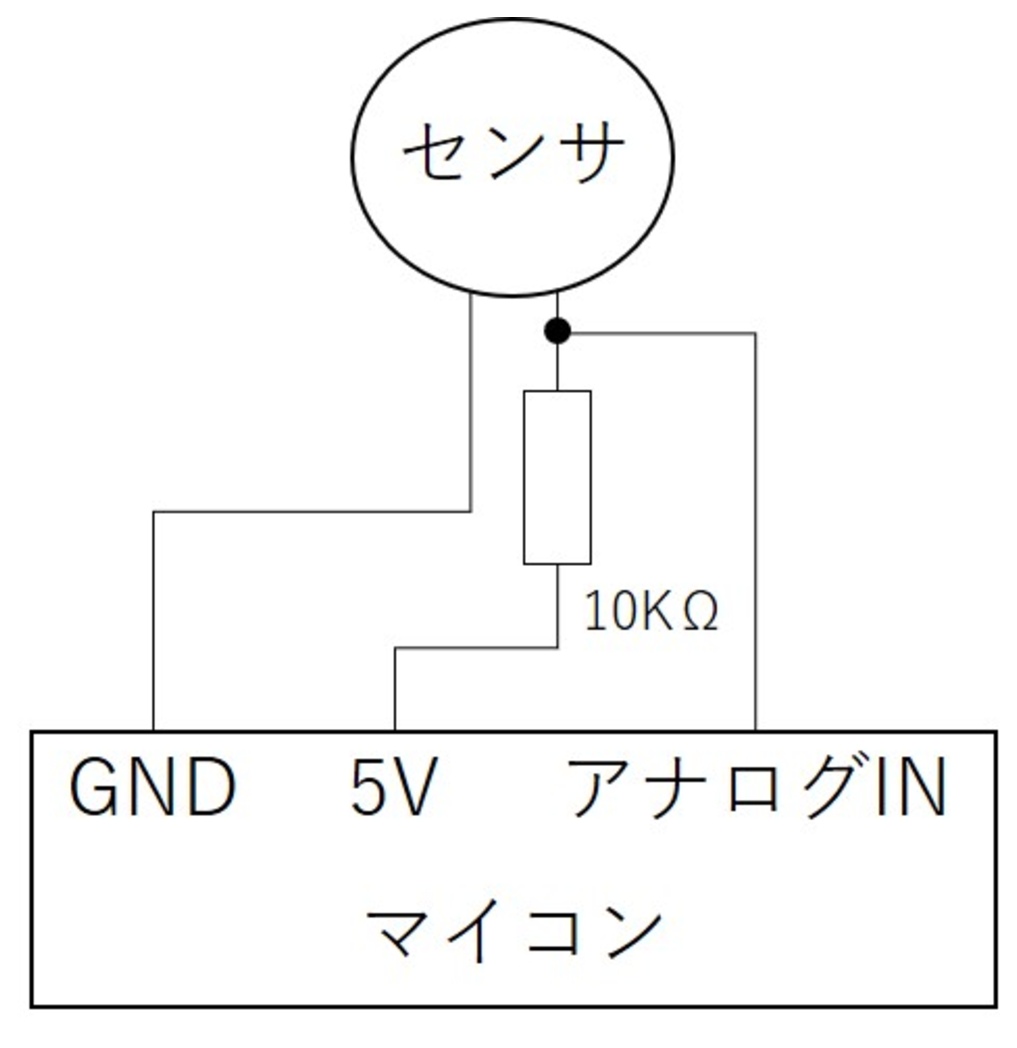
\includegraphics[width=0.5\linewidth]{figure/circuit.eps}
  \end{center}
  \caption{センサ1つあたりの回路図}
  \label{circuit}
\end{figure}

\begin{figure}[!t]
  \begin{center}
    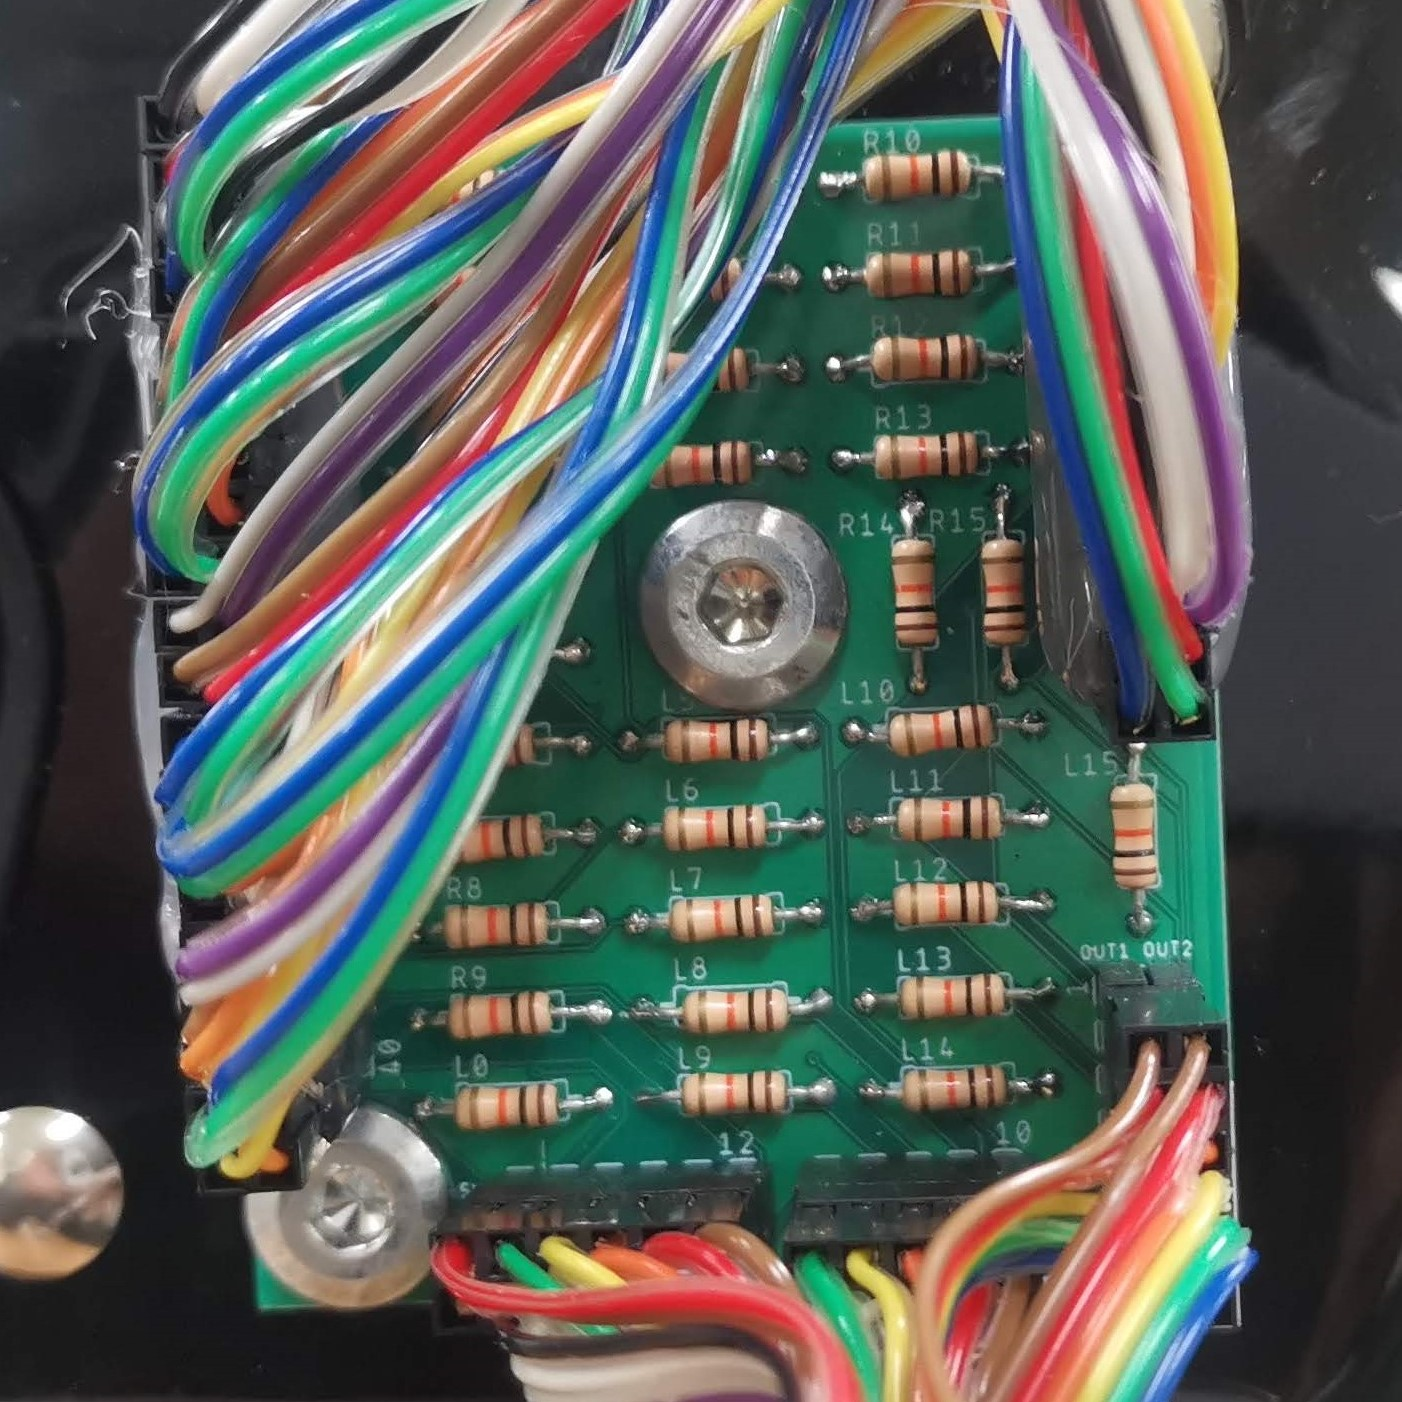
\includegraphics[width=0.5\linewidth]{figure/print.eps}
  \end{center}
  \caption{プリント基板}
  \label{print}
\end{figure}

\section{ソフトウェア}
データの収集にはArduinoIDEを用いてマイコンを制御し,Pythonでセンサデータをコンピュータ上にcsvとして収集するプログラムを作成した.次にデータの解析はPython上でcsvを読み出し,sklearn.covariance.MinCovDetを用いてマハラノビス距離を計算した.そして,計算結果に対し閾値を移動させながら比較,識別しながら評価指標を計算するプログラムを実装した.\par
ここで用いたsklearn.covariance.MinCovDetとは,異常値に対して頑健な共分散行列の推定アルゴリズムであるMinimum Covariance Determinant(以下MCDと表記)を高速化したFast-MCD\cite{fast_mcd}を実装したscikit-learnのライブラリである.
\chapter{評価}
\label{evaluation}
本章では,提案手法の有効性を評価するために行った実験について説明する.

\section{データ収集}
被験者9名(A$\sim$I,全員男性,平均年齢23歳)に実装したヘルメットを装着させ,サンプリングレート約30Hzでセンサデータを収集した.2秒間装着して取り外し再び2秒装着する試行を1セットとして被験者1人あたり10セット,合計20回装着するデータ(2秒$\times$2回$\times$10セット)を収集した.データの収集は1人当たり1日最大4セットとし,複数日に渡ってデータを収集した.センサと頭部のさまざまな位置関係のデータを収集するために,セット間に30分以上の休憩時間を設けた.1回2秒間32次元の装着データの時間平均値を算出し,1回の装着から32次元のベクトルを1サンプル得る.つまり,被験者1人あたり20サンプルを取得した.

\section{結果と考察}
収集したデータに対して,1名を本人,8名を他人として,収集した本人のデータの80\%を登録し,20\%のデータを用いて本人の認証精度を計測した.また,8人すべてのデータを用いて他人の認証精度を計測した.登録データは5分割交差検証を行い評価した.

識別結果の評価指標として,FRR,FAR,EERを用いる.FRR(False Reject Rate:本人棄却率)は誤って本人を他人であると判断し拒否してしまう割合であり,FAR(False Accept Rate:他人受入率)は誤って他人を本人であると判断し認証してしまう割合である.閾値を小さくするほどFRRが増加し,閾値を大きくするほどFARが増加する.FRRとFARはトレードオフの関係にあり,FRRとFARが同値になるときの値をEER(Equal Error Rate:等誤り率)と呼ぶ.通常,EERの値で本人認証の性能を評価し,EERが小さいほど精度が良い.被験者ごとに閾値を変化させてEERを計測した.

各被験者および9人の平均EERを表\ref{EER_num}に,FRRとFARを図\ref{EER}に示す.Totalは被験者全員の平均を示している.
表\ref{EER_num}より被験者A,E,G,IのEERはおおよそ0.01以下と良い結果が得られた.これは,検証に用いたデータセットにおいて,本人は100回に1回以下の割合で認証に失敗し,他人は100回に1回以下の割合で認証を突破することを意味している.文献\cite{face_auth}において,顔認証のEERが0.012であると報告されていることを考慮すると,これらの被験者については同等の性能が得られたといえる.被験者Eについては,他の被験者よりも極めて大きい3000程度のところでFRRとFARが交差している.これは収集した圧力データのサンプルに大きく外れた値が存在したため,そのサンプルが正しく認証されるために閾値を大きくする必要があったからである.

次に精度が良かった被験者C,D,HのEERはおおよそ0.05である.ここで精度の低下の原因を究明するため,収集したすべてのデータに対して主成分分析を行い,第一主成分および第二主成分の2次元に圧縮したデータを2次元平面上にプロットし,目視で確認できるようにした.この結果を図\ref{PCA}に示す.図\ref{PCA}より,被験者Cのデータ群は1サンプルが被験者Iのデータ群と近い位置にあることを除き,他の被験者のデータ群との重なりは見られない.ただし,第一主成分方向の分散が大きく,データの散らばりが精度の低下に影響したと考えられる.被験者D,Hのデータ群は分散が小さいが,互いに大きく重なっており,両者が影響し合って精度が低下したと考えられる.

最も精度が悪かった被験者はB,Fであり,これらの被験者のEERはおおよそ0.095であった.被験者Bのデータ群は分散が小さいが,被験者Iのデータ群との重なりが見られる.しかしながら,検証に用いたデータセットにおける被験者IのEERは0.000であり,誤りなく判別ができていた.したがって,これらのデータ群の重なりは主成分分析で2次元に圧縮した際のデータの損失による影響だと考えられ,重なりは精度の低下に影響していないことが確認できる.一方,被験者Fのデータ群は他の被験者のデータ群との重なりが見られないが,分散が大きい.このデータ群の散らばりの形に注目すると,第一主成分と第二主成分のそれぞれの方向に散らばりが見られる.主成分分析によるデータの丸めの影響を考慮すると,実際のデータ群ではかなり色々な次元の方向にデータが散らばっていると考えられる.この被験者Fのデータの散らばりに影響され,データ群が近くに位置する被験者Bの精度も低下したと考えられる.

被験者全員の平均EERは約0.076という結果であった.被験者ごとのEERに差が見られたことから,さらなる精度の向上を目指すことが可能であると考えられる.

提案手法ではマハラノビス距離を用いて識別を行うため,学習データ数をさらに増やすことで精度の向上が見込まれる.一方で,距離が同じ場合は識別が不可能となってしまう.その場合,提案手法と別の手法で識別を行う必要がある.具体的には,ヘルメットを装着する一連の流れを時系列データとして取得し,その特徴により識別を行う手法が考えられる.この手法が有効であるかを今後検証していく.

\begin{table}[!t]
  \centering
  \caption{被験者ごとのEER}
  \begin{tabular}{c|c} \hline\hline
    被験者 & EER \\ \hline
    A & 0.002 \\
    B & 0.095 \\
    C & 0.050 \\
    D & 0.055 \\
    E & 0.006 \\
    F & 0.094 \\
    G & 0.012 \\
    H & 0.050 \\
    I & 0.000 \\ \hline
    Total & 0.076 \\ \hline
  \end{tabular}
  \label{EER_num}
\end{table}

\begin{figure}[!t]
  \centering
    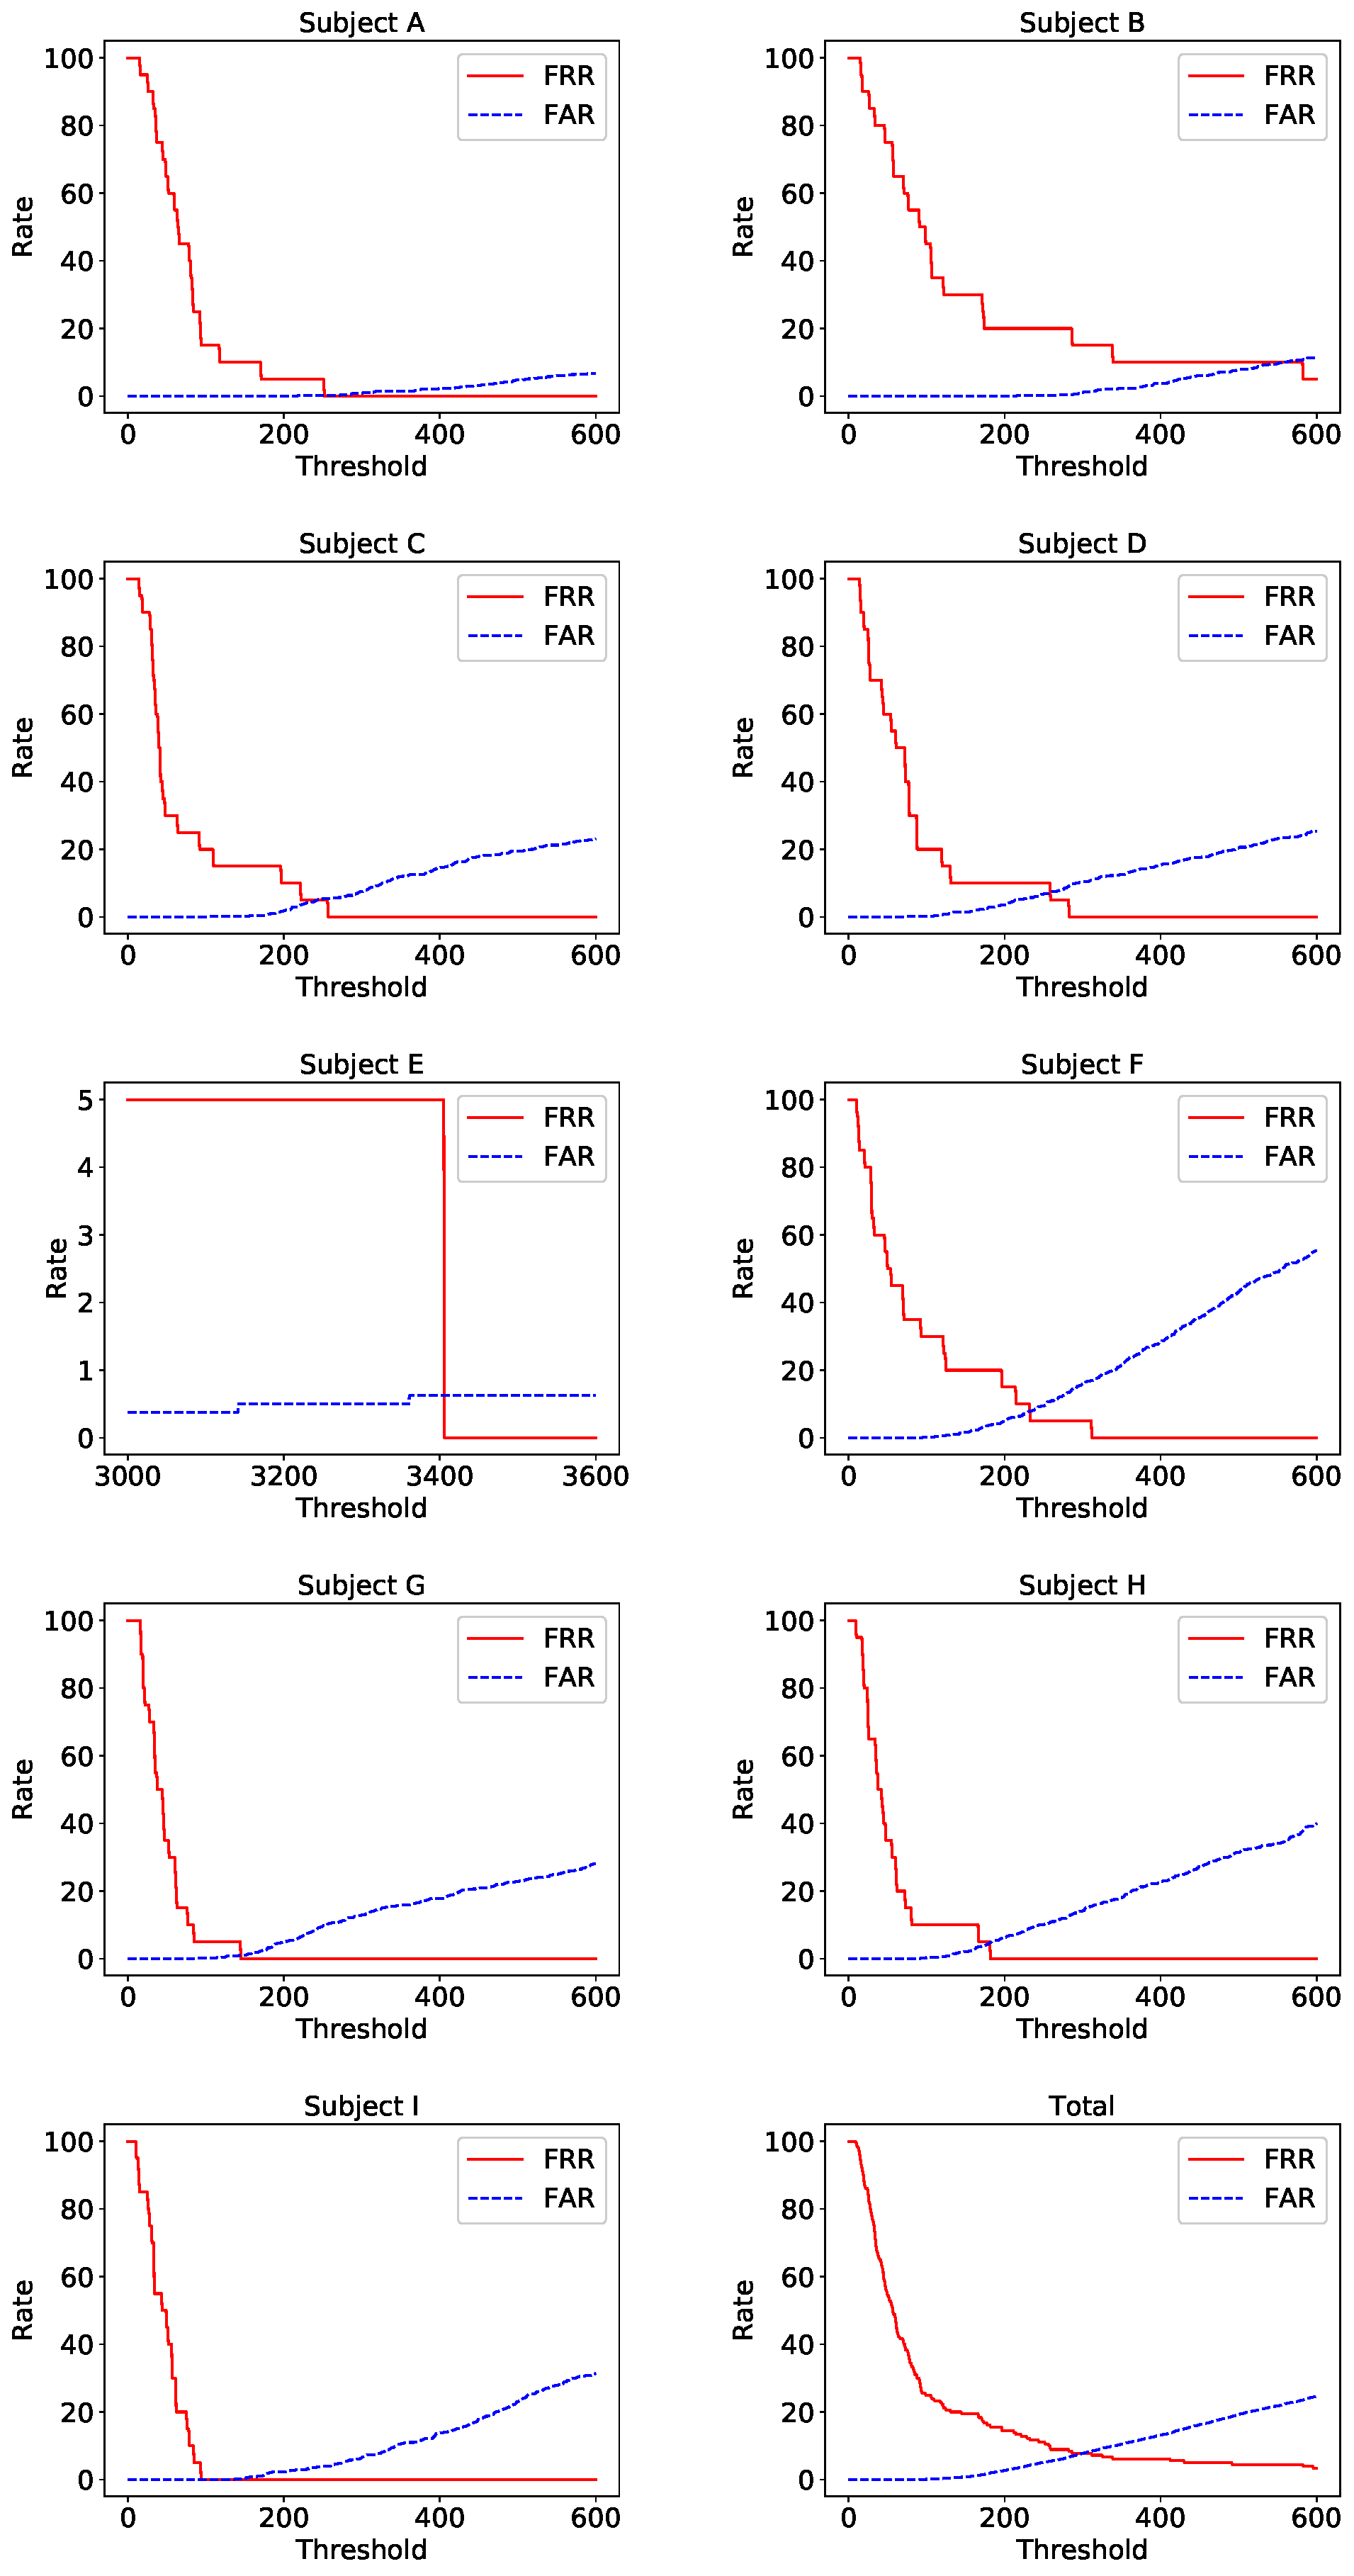
\includegraphics[width=0.70\linewidth]{figure/EER.eps}
  \caption{被験者ごとの判別結果}
  \label{EER}
\end{figure}

\begin{figure}[!t]
  \centering
    \includegraphics[width=1\linewidth]{figure/PCA.eps}
  \caption{PCAによる分析結果}
  \label{PCA}
\end{figure}
\chapter{おわりに}
\label{conclude}
本研究では,圧力センサを内部に取り付けたヘルメットを装着することで頭部の形状を計測し,頭部形状の個人差から二輪車の所有者本人を認証する手法を提案し,プロトタイプデバイスの実装とデータ収集および解析プログラムを作成した.プロトタイプデバイスは市販のフルフェイス型ヘルメットを加工し,圧力センサを取り付けた.実験では,プロトタイプデバイスからデータを取得するためにデータ収集プログラムを作成し,頭部形状データとして被験者9人からそれぞれ2秒間のセンサ値を20回分取得した.解析に用いたプログラムはPythonで実装し,登録データと入力データのマハラノビス距離を計算し,本人認証するか拒否するかの閾値を移動させて認証性能を評価した.評価実験の結果,認証の精度の評価指標であるEERが9名中4名が0.012以下,平均0.076という結果が得られた.この結果より,本手法は本人認証手法として有効であると考えられる.今後はさらなるデータの収集を行い,実環境での提案手法の評価を行う.

\chapter*{謝辞}
本研究全般に関して,懇切なる御指導と惜しみない御助言を頂きました立命館大学情報理工学部情報システム学科村尾和哉准教授に謹んで御礼申し上げます.本研究を推進するにあたり,御指導,御助言,御討論を頂きました立命館大学情報理工学部情報システム学科双見京介助教に衷心より感謝申し上げます.本研究を進めるにあたり,多くの御協力,御助言,御討論を頂きました立命館大学情報理工学部情報システム学科村尾研究室の諸氏に心より感謝申し上げます.最後に,研究生活を送る上で,暖かい御支援と多大なる御理解を頂いた両親を始めとする家族に心からの感謝と御礼を申し上げます.
\addcontentsline{toc}{chapter}{謝辞}

\bibliographystyle{junsrt}
\bibliography{references}

\end{document}